\documentclass[12pt, a4paper, twoside, onecolumn]{article}

\usepackage{cs351_preamble}

% You may want to use \vspace{-1cm} at times to change vertical spacing in a slightly hacky but functional way

\title{CS351 Computer Systems Engineering Project \\ \vspace{0.5cm} Network Switch Design on Field-Programmable Gate Arrays \\ \vspace{0.3cm} \Large{Progress Report}}
\author{1611586}

\begin{document}

\begin{titlepage}
   \begin{center}
       % \vspace*{1.5cm}

      
\includegraphics[width=0.25\textwidth]{warwick_logo_old.png}

      \vspace{1.5cm}
      \textbf{\Large{Network Switch Design on Field-Programmable Gate Arrays}}

      \vspace{1cm}
      \textbf{\large{CS351 Computer Systems Engineering Project}} \\
      \vspace{0.5cm}


      \textbf{\large{Progress Report}}

      \vspace{2.7cm}

      \textbf{Benji Levine} \\
      \vspace{0.1cm}
      \textbf{1611586}

      \vspace{2.7cm}

      Superviser: Dr Suhaib Fahmy

      \vspace{0.8cm}

      Department of Computer Science\\
      University of Warwick

      \vspace{0.7cm}

      2018-19

   \end{center}
\end{titlepage}


\title{CS351 Computer Systems Engineering Project \\ \vspace{0.5cm} Network Switch Design on FPGAs \\ \vspace{0.3cm} \Large{Progress Report}}
\author{1611586}


\tableofcontents
\newpage

\section{Glossary}
\label{glossary}
The following acronyms are used throughout the specification.
\begin{itemize}
  \item \textbf{FPGA}: Field-Programmable Gate Array
  \item \textbf{MTU}: Maximum Transmission Unit
  \item \textbf{OSI model}: Open Systems Interconnection reference model
  \item \textbf{IP}: Internet Protocol
  \item \textbf{TCP}: Transmission Control Protocol
  \item \textbf{ARPANET}: Advanced Research Projects Agency Network
  \item \textbf{DARPA}: Defense Advanced Research Projects Agency (USA)
  \item \textbf{UTP}: Unshielded Twisted Pair
  \item \textbf{SDN}: Software-defined Networking
\end{itemize}

\section{Introduction}
\label{introduction}




\section{Research}
\label{research}

\subsection{Networking}
Since core networking concepts form much of the background for this project, a reasonable amount of time was dedicated to researching these. These are detailed below.

\subsubsection{Network Packets}
\label{network_packets}

A `packet' in networking refers to a unit of data. This term only applies to certain units of data, since data at different stages in network models (see section \ref{network_models}) takes different names. Ultimately, a packet consists of two parts: a set of `headers', and a `payload'. The headers contain metadata about the packet, such as where it was sent from, where it was sent to, or a checksum of the packet used for error checking. A packet tends to have multiple headers, each stacked on top of one another. Each header is used by a different layer of the OSI model (see section \ref{network_models}). When a packet is being constructed, each layer prepends its header to the packet payload before sending it down to the next layer. The payload carries the actual packet data. In most cases, many packets will be required to send a message, since packets have a fixed maximum size. This limit in size is known as the Maximum Transmission Unit (MTU), and for an Ethernet packet, this is 1518 bytes including headers.

\subsubsection{Network Models}
\label{network_models}
The two most commonly used models are the Open Systems Interconnection Reference model (commonly referred to as the OSI model), and the TCP/IP model. Both of these models consist of layers and are intended to allow the detail of the layers beneath the layer you are working at to be abstracted away. This means that, for example, a web server will not need to know any detail about the networking hardware of the server it is running on.

The OSI model was created in 1994 \cite{iec7498_1_1994} and consists of seven layers, shown in table \ref{osi_model}. It has suffered from a few key criticisms, such as the fact that some layers have very little use in most applications, and the complexity of the model can result in large and slow systems. In addition, when the OSI standard was approved, the competing TCP/IP model was being used by most research universities, and so did not receive as much support as might have been expected

The TCP/IP model was developed for ARPANET, a predecessor of the modern internet funded by DARPA. TCP was developed to serve as a protocol for communication within ARPANET from different underlying hardware (such as between satellite packet networks and ground-based radio packet networks). It initially covered both the Internet and Transport layers of what would become the TCP/IP model, however it was suggested to separate the protocol, which resulted in the creation of the Internet Protocol (IP). These protocols went through a number of revisions before arriving at TCP/IP v4, which is still in use today.

\begin{table}[!ht]
  \begin{center}
    \begin{tabularx}{\textwidth}{|c|l|X|}
      \hline
      \textbf{7} & Application & The layer where user programs live. In addition to user specificed programs, there are common applications such as FTP, Telnet (virtual terminal), or e-mail, which operate at the application layer. \\ \hline
      \textbf{6} & Presentation & Provides a set of data transformation services including character conversion, data compression, and data encryption. \\ \hline
      \textbf{5} & Session & Designed to manage an entire conversation, consisting of a number of dialogue units which can be suspended and restarted through synchronisation points. However, client/server communication is based on an asymmetric model, in which one or more client processes can request resources from a server process. \\ \hline
      \textbf{4} & Transport & Provides datagrams for both connection-oriented and connectionless protocols. In a connection-oriented service, the transport layer negotiates a suitable quality of service for the given network and application. This typically includes throughput, transit delay, and error rate among other paramters. \\ \hline
      \textbf{3} & Network & Highest layer within the communication subnet, deals with control issues like routing, congestion control, and error recovery. \\ \hline
      \textbf{2} & Data Link & Provides frames which give addressing, error control, and sequencing, necessary to provide a reliable service. \\ \hline
      \textbf{1} & Physical & Responsible for transporting bits of information. Bandwidth, signal levels, and signal coding methods are specified at this level. \\ \hline
    \end{tabularx}
  \end{center}
\caption{The Open Systems Interconnection Reference model \cite{networks01}}
\label{osi_model}
\end{table}

\begin{table}[!ht]
  \begin{center}
    \begin{tabularx}{\textwidth}{|c|l|X|}
      \hline
      \textbf{4} & Application & Equivalent to the Session, Presentation, and Application layers of the OSI model. The Application layer is used to handle all process to process communication, and includes session establishment, compression, and encryption. \\ \hline
      \textbf{3} & Transport & Equivalent to the Transport layer of the OSI model. The Transport layer includes message segmentation, session multiplexing, and message reordering. \\ \hline
      \textbf{2} & Internet & Equivalent to the Network layer of the OSI model. The Internet layer includes traffic routing, traffic control, and logical addressing. \\ \hline
      \textbf{1} & Link & Equivalent to the Data Link and Physical layers of the OSI model. Provides physical network functions like signal levels, signal coding methods and, error detection. \\ \hline
    \end{tabularx}
  \end{center}
  \caption{The TCP/IP model \cite{tcpip_pearson}}
  \label{tcp_ip_model}
\end{table}

\subsubsection{Packet Switching}
Layers of a model can offer either a connection-oriented or a connectionless service to the layers above. A connection-oriented service involves establishing a connection, using the connection, and then releasing the connection, similar to a landline telephone system. This requires all the parameters for the connection to be specified in advance, which may involve a negotiation between the sender and the receiver.

A connectionless service involves providing every packet with the full source and destination address for the data. Each packet is then sent independently such that each node the packet passes through chooses the next node to send it to. The current node makes this decision by choosing the node that is closest to the packet's final destination from the nodes it is aware of. There are two main switching methods for a connectionless service: ``store-and-forward'' and ``cut-through''. ``Store-and-forward'' involves each intermediate node receiving a message in full before forwarding packets to the next node, while ``cut-through'' does not require an intermediate node to have the entire message before it starts forwarding packets \cite{tanenbaum}.

\subsubsection{Physical Media}
There are different categories of physical media that can be used to transmit data. The two most common types are UTP and optical fibre. UTP consists of two copper wires coated in plastic and twisted together. The wires are twisted partially to keep them together, but also to help cancel out electromagnetic interference between the wires \cite{networks03}. UTP is currently the dominant media, primarily since it has been commercially available for so long.

Optical fibre beats out copper in most categories, only really falling behind when it comes to cost, the price gap between UTP and optical fibre is narrowing \cite{copper_fibre_universal}. Optical fibre has a singicantly higher theoretical maximum bandwidth, is much more durable, and can be used across much longer distances with less signal attenuation \cite{copper_fibre_multicom}. UTP and optical fibre do use different connectors and so it is difficult to take full advantage of the benefits of optical fibre when using the standard ethernet connectors found in most consumer hardware. All of the hardware platforms offered by NetFPGA aside from the NetFPGA 1G \cite{NetFPGA_1G} are designed for optical fibre. %This is discussed further in section \ref{netfpga_research}.

% \subsubsection{Performance}

\subsubsection{Packet Headers}
As mntioned in section \ref{network_packets}, `headers' are used to store metadata about network packets. Each layer of the TCP/IP model prepends an additional header to the data, resulting in a payload with multiple headers attached as shown in figure \ref{segments_packets_frames}. Most protocols have a set header format, making it much easier to extract data from them. As an example, the header for an IPv4 packet is shown in figure \ref{ip_header}. Each row of the header represents 32 bits of data. The \textit{Options} field of the header has a variable length, so the \textit{IHL} field is used to record the length of the IP header. The \textit{Total Length} field represents the total size of the packet in 32 bit words, including both the header and the payload. This information can be used to extract the data from the headers, and to remove the appropriate number of bits in order to read the payload itself. For this project the P4 language \cite{P4} will be used to extract data from packet headers, as will be discussed further in section \ref{p4_research}.
The \textit{Version} field of the IP header refers to which version of the protocol is used by the packet. The most commonly used version is IPv4, however a newer version, IPv6, has been standardised \cite{rfc1883} \cite{rfc8200}. IPv6 was primarily intended to address the issue of addressing in IPv4. Every device on a network using IP requires a unique IP address. When data is being sent to a particular device, its IP address is used at the Internet layer of the TCP/IP model to locate the device. An IPv4 address is 32 bits long, meaning there are a total of 4,294,967,296 IPv4 addresses for a given network. While this is more than enough for any local network, a very large network (such as the internet) does run the risk of hitting this limit. In fact, the internet has now had all of the available addresses allocated \cite{iana_ipv4_address_space_registry}. Comparatively, an IPv6 address is 128 bits long, providing a total of $3.4 \times 10^{38}$ IPv6 addresses. Since IPv6 is not yet widely implemented, it is being considered beyond the scope of this project.

\begin{figure}[h]
	\begin{center}
		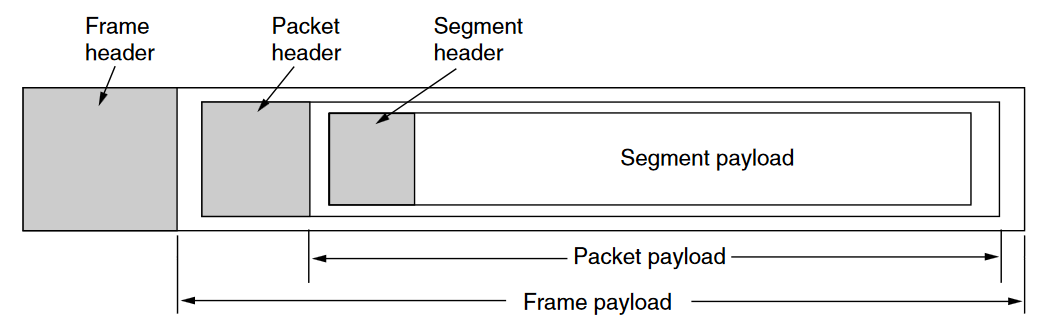
\includegraphics[width=14cm]{frames.png}
	\end{center}
	\caption{Nesting of segments, packets, and frames. \cite{tanenbaum}}
	\label{segments_packets_frames}
\end{figure}

\begin{figure}[h]
	\begin{center}
		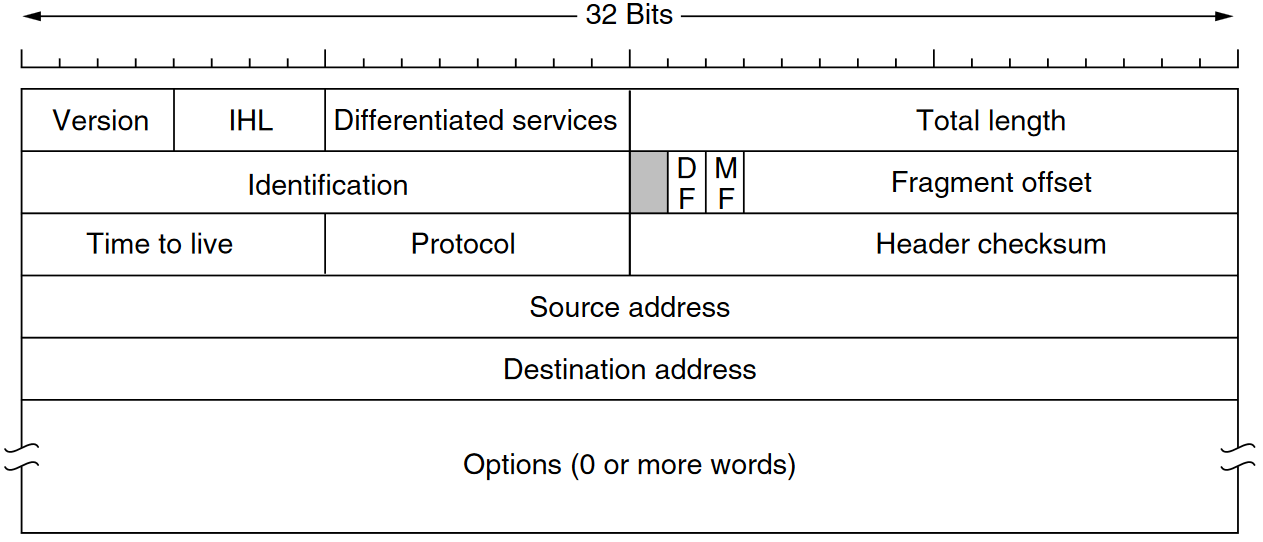
\includegraphics[width=14cm]{ip_header.png}
	\end{center}
	\caption{The IPv4 (Internet Protocol) header. \cite{tanenbaum}}
	\label{ip_header}
\end{figure}

\subsubsection{Software-Defined Networking}
\label{software_defined_networking}
The primary benefit of SDN is that it gives the programmer more direct and clear control over how routing decisions are made. SDN aims to separate the network control, known as the control plane, from the forwarding proces, known as the data plane \cite{software_defined_networking_survey}. The control plane makes decisions about packets which are either destined to or originally from the current host, while the data plane makes decisions about packets which are going through the host. The control plane also maintains the routing table, which is used by both planes to make routing decisions.

\subsection{P4}
\label{p4_research}
P4 is a language for programming the data plane of network devices \cite{P4}. The specification for $P4_{14}$ (the first version of P4) was released in September 2014. This went through a few minor revisions before the specification for $P4_{16}$ (the current version) was released. This project will use $P4_{16}$.

% \subsection{NetFPGA}
% \label{netfpga_research}
%
% \section{Development Technologies}


\section{Future Steps}
The next steps for this project are to begin the implementation of a packet analyser using $P4_{16}$ on a NetFPGA. This will be initially completed using a virtual platform instead of on the NetFPGA directly, since access to the hardware will be limited before the start of Term 2. An updated project timetable is shown in figure \ref{gantt_chart}. This has not changed significantly since the specification document was written. The specification document, along with the original project timetable, can be found in appendix \ref{initial_spec}.

% \section{Timetable}
% \label{timetable}
% \afterpage{
\begin{landscape}
% \hvFloat{figure}{
\begin{figure}[h!]
  \begin{center}
  \scalebox{0.9}{
  \begin{ganttchart}[hgrid, vgrid]{1}{32}
    \gantttitle{Term 1}{10}
    \gantttitle{Christmas}{4}
    \gantttitle{Term 2}{10}
    \gantttitle{Easter}{5}
    \gantttitle{Term 3}{3} \\
    \gantttitlelist{1,...,10}{1}
    \gantttitlelist{1,...,4}{1}
    \gantttitlelist{1,...,10}{1}
    \gantttitlelist{1,...,5}{1}
    \gantttitlelist{1,...,3}{1} \\
    % \ganttgroup{Initial Research}{2}{7} \\
    \ganttbar[name=write_spec]{Write Specification}{1}{2} \\
    \ganttmilestone[name=submit_spec]{Submit Specification}{2} \\
    \ganttbar[name=r_network]{Research Networking Concepts}{3}{3} \\
    \ganttbar[name=r_netfpga]{Research NetFPGA}{4}{4} \\
    \ganttbar[name=r_p4]{Research P4}{5}{6} \\
    \ganttbar[name=write_prog]{Write Progress Report}{7}{9} \\
    \ganttmilestone[name=submit_prog]{Submit Progress Report}{9} \\
    \ganttbar[name=implement_pa_virtual]{Implement a Packet Analyser in a virtual environment}{10}{15} \\
    \ganttbar[name=implement_pa]{Implement a Packet Analyser on NetFPGA}{16}{17} \\
    \ganttbar[name=implement_ps]{Implement a Packet Switcher on NetFPGA}{18}{20} \\
    \ganttbar[name=compare_speed]{Compare latency of NetFPGA switch with conventional switch}{21}{21} \\
    \ganttbar[name=prep_presentation]{Prepare Presentation}{22}{23} \\
    \ganttmilestone[name=presentation]{Presentation}{23} \\
    \ganttbar[name=write_final]{Write Final Report}{24}{31} \\
    \ganttmilestone[name=submit_final]{Submit Final Report}{31} \\
    \ganttlink{write_spec}{submit_spec}
    \ganttlink{submit_spec}{r_network}
    \ganttlink{r_network}{r_netfpga}
    \ganttlink{r_netfpga}{r_p4}
    \ganttlink{r_p4}{write_prog}
    \ganttlink{write_prog}{submit_prog}
    \ganttlink{submit_prog}{implement_pa_virtual}
    \ganttlink{implement_pa_virtual}{implement_pa}
    \ganttlink{implement_pa}{implement_ps}
    \ganttlink{implement_ps}{compare_speed}
    \ganttlink{compare_speed}{prep_presentation}
    \ganttlink{prep_presentation}{presentation}
    \ganttlink{presentation}{write_final}
    \ganttlink{write_final}{submit_final}
  \end{ganttchart}}
  \caption{Gantt Chart of Project Timetable}
  \label{gantt_chart}
\end{center}
\end{figure}%{Gantt Chart of Project Timetable}
\end{landscape}
% }

% \end{changemargin}

\section{Conclusion}


\bibliographystyle{ieeetr}
\bibliography{bibliography}

% \begin{appendices}
%   \section{Initial Specification}
%   \label{initial_spec}
%   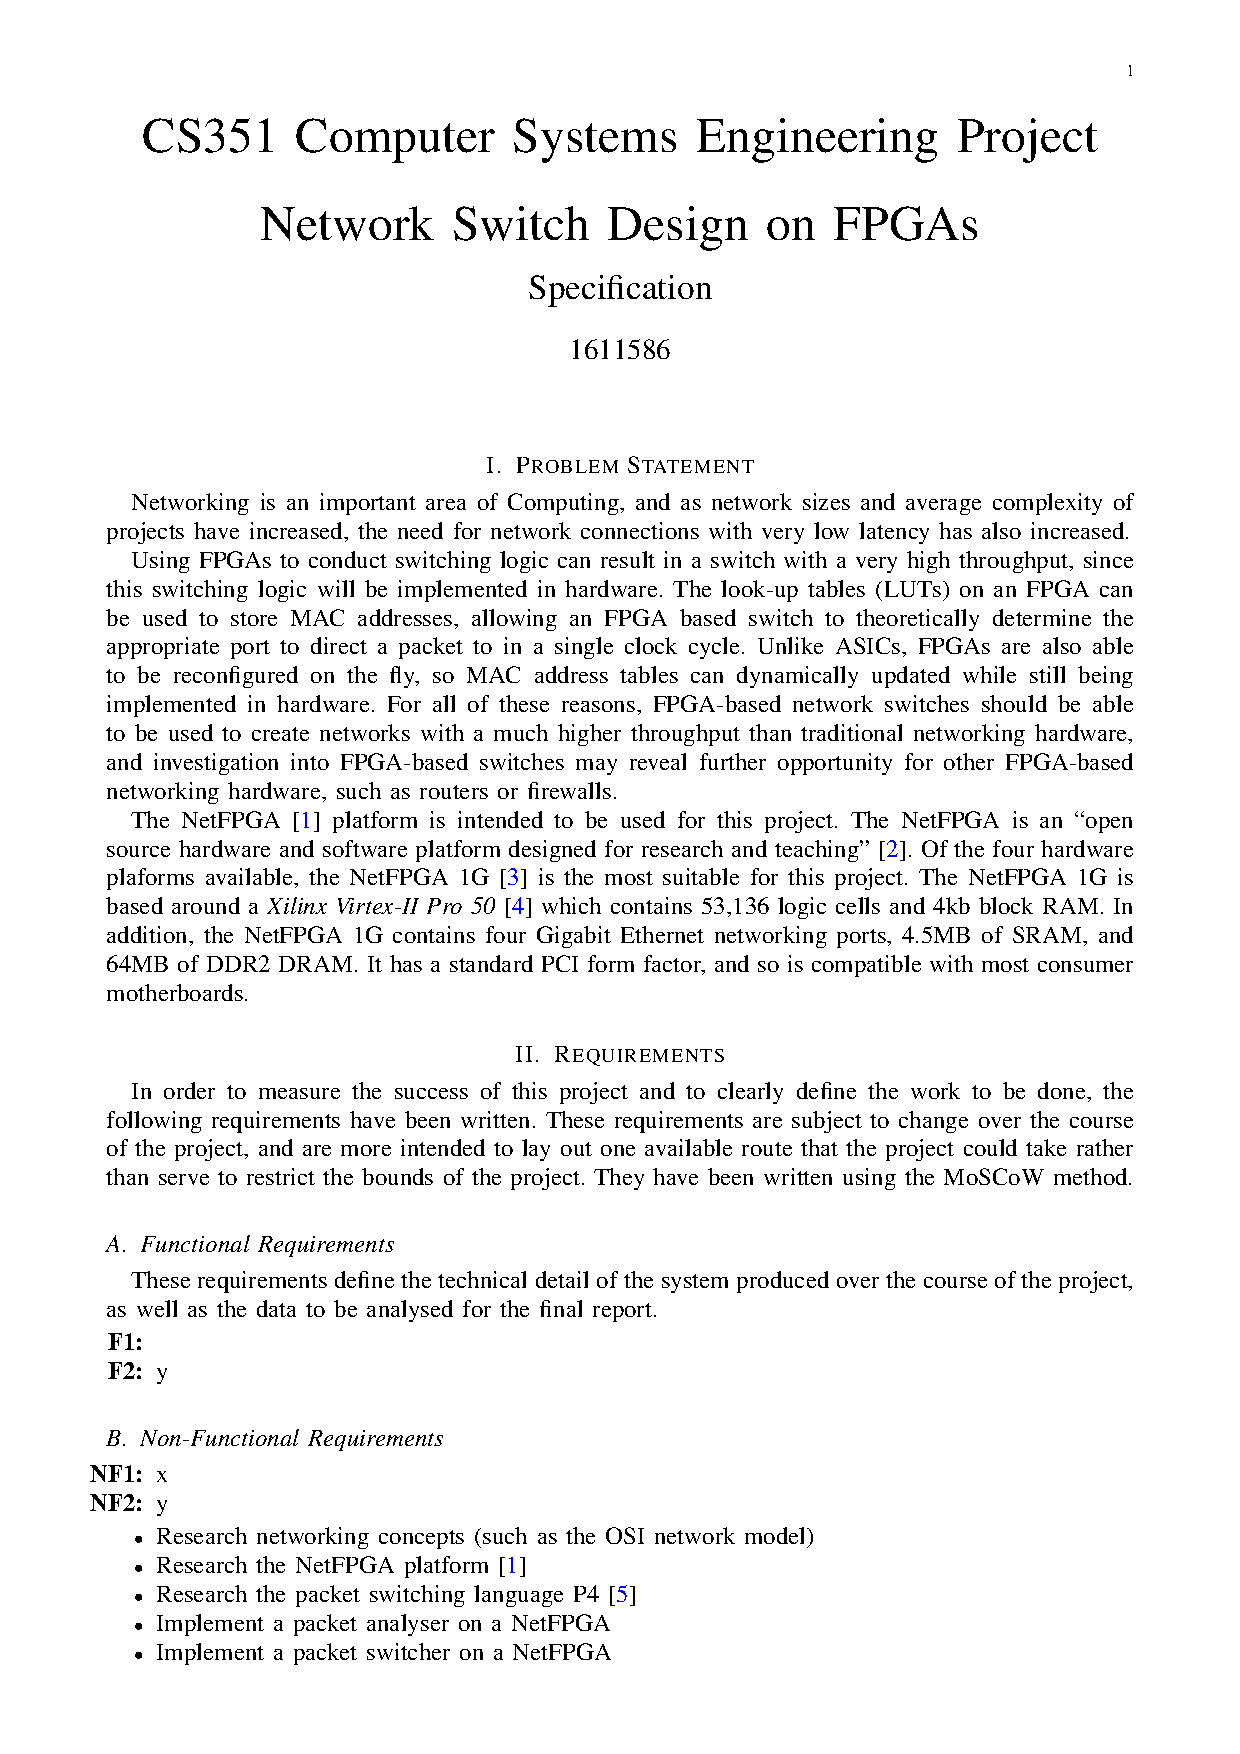
\includepdf[pages=-]{specification.pdf}
%   % \documentclass[12pt, a4paper, twoside, onecolumn]{article}

%% Language and font encodings
\usepackage[english]{babel}
\usepackage[utf8x]{inputenc}
\usepackage[T1]{fontenc}
\usepackage{mathptmx}

%% Sets page size and margins
\usepackage[a4paper,top=2cm,bottom=1.6cm,left=1.8cm,right=1.8cm,marginparwidth=2cm]{geometry}

%% Useful packages
\usepackage{amsmath}
\usepackage{graphicx}
\usepackage{pgfgantt}
\usepackage{url}
\usepackage{xparse}
\usepackage{listings}
\usepackage[colorlinks=true, allcolors=blue]{hyperref}
\usepackage{caption}
\usepackage{lscape}
\usepackage{enumitem}

\hypersetup{
    colorlinks = false
}

%% Section Numbering
%\setcounter{secnumdepth}{0} % no sections will be numbered
%\setcounter{secnumdepth}{1} % only sections will be numbered
%\setcounter{secnumdepth}{2} % sections and subsections will be numbered
%\setcounter{secnumdepth}{3} % sections, subsections and subsubsections will be numbered

%% TrueType font for code. use \codeword{} around sections of code in your document
\NewDocumentCommand{\codeword}{v}{
  \texttt{\textcolor{black}{#1}}
}

% You may want to use \vspace{-1cm} at times to change vertical spacing in a slightly hacky but functional way

\title{CS351 Computer Systems Engineering Project \\ \vspace{0.5cm} Network Switch Design on Field-Programmable Gate Arrays \\ \vspace{0.3cm} \Large{Specification}}
\author{1611586}

\begin{document}

\begin{titlepage}
   \begin{center}
       \vspace*{1.5cm}

      
\includegraphics[width=0.25\textwidth]{warwick_logo_old.png}

      \vspace{1.5cm}
      \textbf{Network Switch Design on FPGAs}

      \vspace{1.5cm}
      \textbf{CS351 Computer Systems Engineering Project} \\
      \vspace{0.5cm}


      \textbf{Specification}

      \vspace{4cm}

      \textbf{Benji Levine}

      \vspace{4cm}

      Superviser: Dr Suhaib Fahmy

      \vspace{0.8cm}

      Department of Computer Science\\
      University of Warwick

      \vspace{0.7cm}

      2018-19

   \end{center}
\end{titlepage}


\title{CS351 Computer Systems Engineering Project \\ \vspace{0.5cm} Network Switch Design on FPGAs \\ \vspace{0.3cm} \Large{Specification}}
\author{1611586}


\tableofcontents
\newpage

\section{Glossary}
\label{glossary}
The following acronyms are used throughout the specification:
\begin{itemize}
  \item \textbf{FPGA}: Field-Programmable Gate Array
  \item \textbf{ASIC}: Application-Specific Integrated Circuit
  \item \textbf{LUT}: Look-Up Table
\end{itemize}

\section{Problem Statement}
\label{problem_statement}
Networking is an important area of Computing, and as network sizes and average complexity of projects have increased,
the need for network connections with very low latency has also increased.

Using FPGAs to conduct switching logic can result in a switch with a very high throughput, since this switching logic will be implemented in hardware. The look-up tables (LUTs) on an FPGA can be used to store MAC addresses, allowing an FPGA based switch to theoretically determine the appropriate port to direct a packet to in a single clock cycle. Unlike ASICs, FPGAs are also able to be reconfigured on the fly, so MAC address tables can dynamically updated while still being implemented in hardware.
For all of these reasons, FPGA-based network switches should be able to be used to create networks with a much higher throughput than traditional networking hardware, and investigation into FPGA-based switches may reveal further opportunity for other FPGA-based networking hardware, such as routers or firewalls.

The NetFPGA \cite{NetFPGA} platform is intended to be used for this project. The NetFPGA is an ``open source hardware and software platform designed for research and teaching'' \cite{NetFPGA_about}. Of the four hardware plaforms available, the NetFPGA 1G \cite{NetFPGA_1G} is the most suitable for this project. The NetFPGA 1G is based around a \textit{Xilinx Virtex-II Pro 50} \cite{virtex2-pro} which contains 53,136 logic cells and 4kb block RAM. In addition, the NetFPGA 1G contains four Gigabit Ethernet networking ports, 4.5MB of SRAM, and 64MB of DDR2 DRAM. It has a standard PCI form factor, and so is compatible with most consumer motherboards.

\section{Requirements}
\label{requirements}
In order to measure the success of this project and to clearly define the work to be done, the following requirements have been written. These requirements are subject to change over the course of the project, and are more intended to lay out one available route that the project could take rather than serve to restrict the bounds of the project. They have been written using the MoSCoW method.

\subsection{Functional Requirements}
\label{functional_requirements}

These requirements define the technical detail of the system produced over the course of the project, as well as the data to be analysed for the final report.
\begin{enumerate}[label=\textbf{F\arabic*:}]
  \item The system \textbf{must} be able to analyse packets at layer 2 of the OSI network model
  \item The system \textbf{must} be able to send packets to the correct port based on MAC addresses
  \item The system \textbf{must} be able to store MAC address tables
  \item The system \textbf{must} be able to keep MAC address tables up to date
  \item The average latency of the system \textbf{must} be measured
  \item The throughput of the system \textbf{must} be measured
  \item The system \textbf{should} be able to analyse packets at layer 3 of the OSI network model
  \item The system \textbf{could} be able to analyse packets at layer 7 of the OSI network model
  \item The system \textbf{could} be able to detect basic network attacks (such as SYN Flooding \cite{rfc4987})
  \item The system \textbf{could} implement features of a basic firewall (such as packet filtering \cite{rfc2979})
\end{enumerate}

\subsection{Non-Functional Requirements}
\label{non_functional_requirements}
\begin{enumerate}[label=\textbf{NF\arabic*:}]
  \item The system \textbf{should} be scalable
  \item All code for the system \textbf{should} be well documented and maintainable
  \item The system \textbf{should} be efficient
\end{enumerate}

\section{Objectives}
\label{objectives}

\begin{itemize}
  \item Research networking concepts (such as the OSI network model)
  \item Research the NetFPGA platform \cite{NetFPGA}
  \item Research the packet switching language P4 \cite{P4}
  \item Implement a packet analyser on a NetFPGA
  \item Implement a packet switcher on a NetFPGA
  \item Test throughput and latency of switching packets using the NetFPGA packet switcher
  \item Test throughput and latency of switching packets using a conventional network switch
  \item Compare performance of NetFPGA packet switcher to conventional network switch
  \item Write up performance comparison
\end{itemize}

\section{Project Management}
\label{project_management}

\subsection{Methods}
\label{methods}
This project will use an agile methodology so that it can adapt to changes which arise during the project. Since the research and implementation stages of the project will contribute to confirming the direction the project will take, this flexibilty is important. In addition, git \cite{git} will be used to track changes in both written documents and any code developed for the project, such as any P4 or Verilog code. Repositories will be set up in git for the different areas of the project, and these repositories will be stored primarily on an online GitHub \cite{github} server and will be backed up regularly. A Gantt chart (shown in figure \ref{gantt_chart}) has been constructed to show an outline of the project timetable, and is intended to be flexible to changes arising during the course of the project.

\subsection{Timetable}
\label{timetable}

\begin{landscape}
\begin{figure}
  \begin{center}
  \begin{ganttchart}[hgrid, vgrid]{1}{32}
    \gantttitle{Term 1}{10}
    \gantttitle{Christmas}{4}
    \gantttitle{Term 2}{10}
    \gantttitle{Easter}{5}
    \gantttitle{Term 3}{3} \\
    \gantttitlelist{1,...,10}{1}
    \gantttitlelist{1,...,4}{1}
    \gantttitlelist{1,...,10}{1}
    \gantttitlelist{1,...,5}{1}
    \gantttitlelist{1,...,3}{1} \\
    % \ganttgroup{Initial Research}{2}{7} \\
    \ganttbar[name=write_spec]{Write Specification}{1}{2} \\
    \ganttmilestone[name=submit_spec]{Submit Specification}{2} \\
    \ganttbar[name=r_network]{Research Networking Concepts}{3}{3} \\
    \ganttbar[name=r_netfpga]{Research NetFPGA}{4}{4} \\
    \ganttbar[name=r_p4]{Research P4}{5}{6} \\
    \ganttbar[name=write_prog]{Write Progress Report}{7}{9} \\
    \ganttmilestone[name=submit_prog]{Submit Progress Report}{9} \\
    \ganttbar[name=implement_pa]{Implement a Packet analyser on NetFPGA}{10}{16} \\
    \ganttbar[name=implement_ps]{Implement a Packet Switcher on NetFPGA}{17}{20} \\
    \ganttbar[name=compare_speed]{Compare latency of NetFPGA switch with conventional switch}{21}{21} \\
    \ganttbar[name=prep_presentation]{Prepare Presentation}{22}{23} \\
    \ganttmilestone[name=presentation]{Presentation}{23} \\
    \ganttbar[name=write_final]{Write Final Report}{24}{31} \\
    \ganttmilestone[name=submit_final]{Submit Final Report}{31} \\
    \ganttlink{write_spec}{submit_spec}
    \ganttlink{submit_spec}{r_network}
    \ganttlink{r_network}{r_netfpga}
    \ganttlink{r_netfpga}{r_p4}
    \ganttlink{r_p4}{write_prog}
    \ganttlink{write_prog}{submit_prog}
    \ganttlink{submit_prog}{implement_pa}
    \ganttlink{implement_pa}{implement_ps}
    \ganttlink{implement_ps}{compare_speed}
    \ganttlink{compare_speed}{prep_presentation}
    \ganttlink{prep_presentation}{presentation}
    \ganttlink{presentation}{write_final}
    \ganttlink{write_final}{submit_final}
  \end{ganttchart}
  \caption{Gantt Chart of Project Timetable}
  \label{gantt_chart}
\end{center}
\end{figure}
\end{landscape}


\section{Resources}
\label{resources}
This project will use a number of different resources, including hardware, software, and languages. These are listed below.
\begin{itemize}
  \item git \cite{git}
    \begin{itemize}
      \item git will be used for version control of all code and documents
    \end{itemize}
  \item GitHub \cite{github}
    \begin{itemize}
      \item Will be used as an external server to store code and documents, as well as an interface to git
    \end{itemize}
  \item NetFPGA \cite{NetFPGA}
    \begin{itemize}
      \item Will be used as the platform on which a switch is developed
    \end{itemize}
  \item P4 \cite{P4}
    \begin{itemize}
      \item Will be used to implement packet switching on the NetFPGA
    \end{itemize}
  \item LaTeX \cite{latex}
    \begin{itemize}
      \item Will be used to write and format all documents
    \end{itemize}
  \item Atom \cite{atom}
    \begin{itemize}
      \item Will be used as an editor to write code
    \end{itemize}
\end{itemize}


\bibliographystyle{ieeetr}
\bibliography{bibliography}

\end{document}

% \end{appendices}

\end{document}
